\documentclass[a4paper]{article}
\usepackage{amsfonts}
\usepackage{amsmath}
\usepackage{amssymb}
\usepackage{graphicx}     

\begin{document}
  
\noindent \large Auteur: Thomas Eertmans \\
\noindent \large Studierichting: Informatica\\
\noindent \large Oefeningenreeks 3E nr. 2\\

\medskip

\normalsize

$s(t) = t^3 - 6t^2 + 9t$ \\

2.1) Zoek de snelheid op tijdstip $t$.\\

$s'(t) = 3t^2 - 12t + 9$ \\

2.2) Wat is de snelheid na 2 seconden? Na 4 seconden?\\

$s'(2) = 3 \cdot 2^2 - 12 \cdot 2 + 9 = -3$ \\

$s'(4) = 3 \cdot 4^2 - 12 \cdot 4 + 9 = 9$ \\

2.3) Wanneer is het deeltje in rust?\\

$3t^2 - 12t + 9 = 0$ \\

$D = 144 - 4 \cdot 3 \cdot 9 = 36$ \\

$t_{1,2} = \dfrac{12 \pm 6}{6} = 3$ en $1$ \\

2.4) Wanneer beweegt het deeltje volgens de positieve richting van de as?\\

$\begin{array}{r | c c c c c c c}
x & -\infty & & 1 & & 3 & & +\infty \\ \hline
f'(x) & & + & & - & & + \\ 
f(x) & & \nearrow & M & \searrow & m & \nearrow \\
\end{array}$ \\

De functie bereikt een lokaal maximum in 1, met $s(1) = 4$, en een lokaal minimum in 3, met $s(3) = 0$. Het deeltje beweegt volgens de positieve zin van de as als $s(t) < 1$ of $s(t) > 3$ \\

2.5) Teken en diagram om de beweging van het deeltje te illustreren.\\

\begin{figure}[h]
\centering
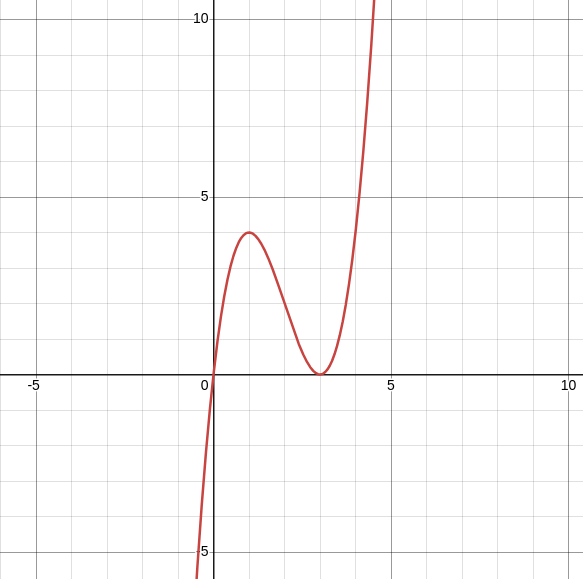
\includegraphics[width = 7cm]{3E-2-thomas.eertmans.INF.png}
\end{figure}

2.6) Wat is de afstand die het eetlje aflegt in de eerste vijf seconden?\\

$s(1) = 4$ , $|s(3) - s(1)| = 4$ , $|s(5) - s(3)| = 20$ \\ 

$= 4 + 4 + 20 = 28$



\begin{thebibliography}{999}
\bibitem{a} Mathijs Pittoors, 3F-1.11-mathijs.pittoors.INF.tex
\end{thebibliography}
\end{document} 
